\documentclass[a4paper,12pt]{article}

\usepackage[dutch]{babel}
\usepackage{fancyhdr}
\usepackage{graphicx}
\usepackage[pdftex,bookmarks=true]{hyperref}
\usepackage[utf8]{inputenc}
\usepackage{fullpage}
\usepackage{parskip}
\usepackage{float}
\usepackage{subcaption}
\usepackage{tabto}

\title{Samenvatting Onderzoekstechnieken \\ \large TIN 2 - HoGent}
\author{Lorenz Verschingel}

\begin{document}
\maketitle
\section{Het onderzoeksproces}
\subsection{De wetenschappelijke methode}
Aan de hand van \textbf{empirisch onderzoek} zijn we geïnteresseerd in volgende zaken:

\begin{enumerate}
\item Exploratie
\item Beschrijving
\item Voorspelling
\item Controle
\end{enumerate}

Het onderzoeksproces verloop normaal gezien als volgt:

\begin{enumerate}
\item Formuleren

Wat is de onderzoeksvraag
\item Exacte informatie behoefte definiëren

Welke specifieke vragen moeten we stellen
\item Uitvoeren onderzoek

Enquêtes, simulaties\dots
\item Verwerken gegevens

Statistische software
\item Analyseren gegevens

Uitvoeren statistische methodes
\item Conclusie schijven

Schrijven onderzoeksverslag
\end{enumerate}

\subsection{Basisconcepten in onderzoek}
\subsubsection{Variabelen en waarden}
Een variabele is een eigenschap van een object waardoor we objecten van elkaar kunnen onderscheiden.

Een waarde is een specifieke eigenschap, een invullen voor een variabele.

\subsubsection{Meetniveaus}
De kwalitatieve schalen zijn:

\NumTabs{6}
\begin{enumerate}
\item 	Nominaal:
		\tab{Categorieën}
		\tab{geslacht, ras, land\dots}
\item	Ordinaal:
		\tab{Volgorde}
		\tab{militaire rang, opleidingsniveau\dots}
\end{enumerate}

De kwantitatieve schalen zijn:
\NumTabs{6}
\begin{enumerate}
\item 	Interval:
		\tab{Meting: }
		\tab{nulpunt is onbelangrijk}
		\tab{graden Celsius}
\item	Ratio:
		\tab{Meting:}
		\tab{t.o.v. absoluut nulpunt}
		\tab{meter, Joule, kilogram}
\end{enumerate}

\subsubsection{Verbanden tussen variabelen}
Er is een verband tussen variabelen als hun waarde systematisch veranderen.

Men is vooral op zoek naar oorzakelijke verbanden:
\begin{itemize}
\item Frustratie leidt tot aggressie
\item Alcohol leidt tot minder oplettendheid
\end{itemize}
De oorzaak is hierbij de onafhankelijke variabele.

Het gevolg is de afhankelijke variabele.

Hierbij moet men wel opletten. Een verband tussen variabelen duidt niet noodzakelijk op een oorzakelijk verband.

\section{Analyse van 1 variabele}
\subsection{Beschrijvende statistiek}
\subsubsection{Centrummaten}
Het \textbf{gemiddelde} is de som van alle waarden gedeeld door het aantal waarden.

Om de \textbf{mediaan} te vinden, sorteert men de waarden en kiest men dan het middelste nummer.
Bij een even aantal getallen neemt men het gemiddelde van de twee middelste.

De \textbf{modus} is het vaakst voorkomende getal in een reeks getallen.
Als men niet onmiddellijk de modus kan aflezen kan men gebruik maken van ranges. Deze ranges zijn dan modale klassen.

\subsubsection{Spreidingsmaten}
Het \textbf{bereik} van een reeks getallen is de absolute waarde van het verschil tussen het grootste en het kleinste getal in de reeks: $|x_{min} - x_{max}|$

De \textbf{kwartielen} van een gesorteerde reeks getallen zijn de waarden die de lijst in vier gelijke delen verdeelt.
Elk deel vormt dus een kwart van de dataset.
Men spreekt van een eerste, tweede en derde kwartiel genoteerd als respectievelijk $Q_1$, $Q_2$, $Q_3$. Hierbij is $Q_2$ de mediaan.

De \textbf{variantie} is het gemiddelde gekwadrateerde verschil tussen de elementen van de dataset en zijn gemiddelde:
$\sigma^2 = \frac{1}{n}\sum^n_i (\mu-x_i)^2$

De \textbf{standaardafwijking} is hde vierkantswortel van de variantie.

\subsection{Eenvoudige grafieken}
\subsubsection{Cirkeldiagram}
Voordelen:
\begin{itemize}
\item Met percentages rond 20\% kan men makkelijk verduidelijken t.o.v. de volledige dataset.
\end{itemize}
Nadelen:
\begin{itemize}
\item Vergelijking op basis van de hoek.
\item De figuur wordt onduidelijk als er veel categorieën zijn.
\end{itemize}
Men gebruik best zo weinig mogelijk een cirkeldiagram.

\subsubsection{Staafdiagram}
Voordelen:
\begin{itemize}
\item Categorieën zijn makkelijk te vergelijken.
\item Per categorie zijn meerdere staven mogelijk.
\end{itemize}

\subsubsection{Boxplot}
Voordelen:
\begin{itemize}
\item Snelle manier om data te inspecteren en verschillende datasets te vergelijken.
\end{itemize}

\subsection{Interpretatie van grafieken}
\begin{figure}[H]
\centering
\begin{subfigure}{.49\textwidth}
  \centering
  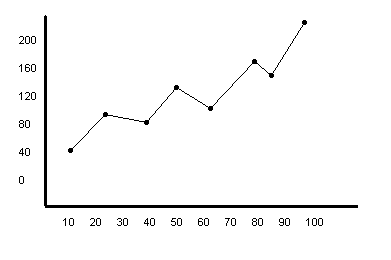
\includegraphics[width=.9\linewidth]{img/Hoofdstuk_2/data-ambiguiteit.png}
  \caption{Data-ambiguïteit}
  \label{fig:data-ambiguiteit}
\end{subfigure}
\begin{subfigure}{.49\textwidth}
  \centering
  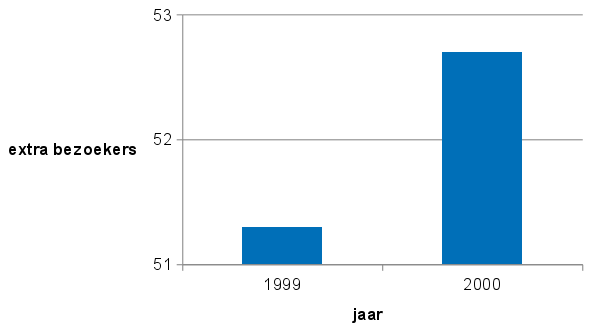
\includegraphics[width=.9\linewidth]{img/Hoofdstuk_2/data_distortion.png}
  \caption{Data distortion}
  \label{fig:datadistortion}
\end{subfigure}
\begin{subfigure}{.49\textwidth}
  \centering
  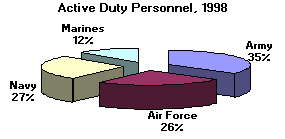
\includegraphics[width=.9\linewidth]{img/Hoofdstuk_2/data_distraction_1.png}
  \caption{Data distraction 1}
  \label{fig:datadistraction1}
\end{subfigure}
\begin{subfigure}{.49\textwidth}
  \centering
  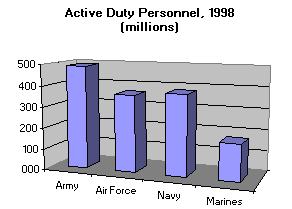
\includegraphics[width=.9\linewidth]{img/Hoofdstuk_2/data_distraction_2.png}
  \caption{Data distraction 2}
  \label{fig:datadistraction2}
\end{subfigure}
\caption{Valkuilen bij het interpreteren van grafieken}
\label{fig:ValkuilenGrafieken}
\end{figure}

\subsubsection{Data-ambiguïteit}
Data-ambiguïteit betekent vergeten aan te duiden wat de data betekent.
Zie figuur~\ref{fig:data-ambiguiteit}.

Enkele tips om dit te voorkomen:
\begin{itemize}
\item Benoem de assen
\item Geef een duidelijk titel
\item Benoem de meeteenheid (en evt. de grootorde)
\item Voeg een bijschrif toe met uitleg over de grafiek
\end{itemize}

\subsubsection{Data distortion}
Data distortion betekend dat men verkeerde conclusies kan trekken uit een grafische voorstelling.
Zie figuur~\ref{fig:datadistortion}: merk hierbij op dat de as niet op nul begint en er maar 3 waarden worden weergegeven.

\subsubsection{Data distraction}
Dit betekent dat de grafiek te veel toeters en bellen bevat.
Men moet de \textit{inkt to data ratio} beperken.
De figuren~\ref{fig:datadistraction1} en ~\ref{fig:datadistraction2} zijn hier voorbeelden van.

\section{Analyse van 2 variabelen}
\subsection{Bivariatie analyse}

\subsection{Kruistabellen en Cramér's V}
Een kruistabel wordt als volgt opgesteld:
\NumTabs{6}
\begin{enumerate}
\item	Percenteer:
		\tab{}
		\tab{Deel de cel door het kolomtotaal}		
\item	Bepaal de schatter 
		\tab{$e=\frac{kolomtotaal \times rijtotaal}{n}$}
		\tab{n: totaal aantal}
\item	Bepaal het verschil
		\tab{$cel - e$}
\item	Kwadrateren en normeren
		\tab($cel = \frac{verschil^2}{e}$)
\end{enumerate}
$\chi^2=\sum\frac{(a-e)^2}{e}$ 

$V = \sqrt{\frac{\chi^2}{n \times (k-1)}}$
met: {$n = totaal$ en $k = min(\#rijen,\#kolommen)$}

Cramér's V is een maat die aanduidt hoe sterk de samenhang is tussen twee nominale variabelen.
Dit getal ligt altijd tussen 0 en 1.
\begin{table}[H]
\centering
\begin{tabular}{|r|r|}
\hline
Waarde & Interpretatie\\
\hline
0 & Geen samenhang\\
0.1 & zwakke samenhang\\
0.25 & redelijk sterke samenhang\\
0.5 & sterke samenhang\\
0.75 & zeer sterke samenhang\\
1 & volledige samenhang\\
\hline
\end{tabular}
\caption{Interpretatie van Cramér's V}
\label{tab:interpretatieCramersV}
\end{table}

\subsection{Regressie}
Bij regressie gaan we proberen een consistente en systematische koppeling tussen variabelen te vinden.

\begin{itemize}
\item	\textbf{Niet-monotoon}: aanwezigheid (of afwezigheid) van de ene variabele gerelateerd aan de aanwezigheid (of afwezigheid) van een andere variabele.
\item	\textbf{Monotoon}: algemene richting van de samenhang tussen de twee variabelen kan aangeduid worden.
\end{itemize}

\subsubsection{Lineaire regressie}
Een lineair verband is een rechtlijnige samenhang tussen een onafhankelijke en afhankelijke variabele, waarbij kennis van de onafhankelijke variabele kennis over de afhankelijke variabele geeft.

\textsc{Kleinste kwadranten methode}

We proberen een rechte te vinden van de vorm $y=\beta_0+\beta_1x$

Hierbij geldt:

$\beta_1 = 
\frac
{\sum^n_{i=1}(x_i-\overline{x})(y_i-\overline{y})}
{\sum^n_{i=1}(x_i - \overline{x})^2}$

$\beta_0 = \overline{y} - \beta_1 \overline{x}$

Kwadraten omdat kleine verschillen minder in rekening moeten gebracht worden dan grote verschillen.
	
Je kan altijd een kleinste kwadratenmethode uitvoeren ==> Dit is daarom wel niet altijd goed.

\subsection{Correlatiecoëfficiënt en determinatiecoëfficiënt}
De Pearson correlatiecoëfficiënt is een maat voor de sterkte van de lineaire samenhang tussen x en y.

De determinatiecoëfficiënt ($R^2$) verklaart het percentage van de variantie van de waargenomen waarden t.o.v. de regressierechte.

\subsubsection{Covariantie}
$cov(x,y) = \sum^n_i 
\frac
{(x_i-\overline{x})(y_i-\overline{y})}
{n}$

$R= \frac{cov(x,y}{\sigma_x\sigma_y}
=
\frac
{cov(x,y)}
{\sqrt{\frac{(x-\overline{x})^2}{n}\times \frac{(y-\overline{y})^2}{n}}}=
\frac{\sum(x-\overline{x})(y-\overline{y})}
{\sqrt{(\sum (x-\overline{x})^2} \times \sqrt{(\sum (y-\overline{y})^2}}$

\section{Steekproefonderzoek}
\subsection{Steekproefonderzoek}
De verzameling van alle objecten of personen waar men in geïnteresseert is en onderzoek wil naar doen, heet de \textit{populatie}.

Wanneer met een subgroep uit een populatie gaat onderzoeken, dan noemen we die groep een \textit{steekproef}.

Om tot een steekproef te komen neemt men de volgende stappen:
\begin{enumerate}
\item Definitie van de populatie
\item Bepalen van het steekproefkader
\item Budget en tijd
\end{enumerate}

Een \textit{gestratificeerde steekproef} is proportioneel als het aandeel van de subpopulatie in de steekproef gelijk is aan het aandeel van de subpopulatie in de populatie als geheel.

\begin{enumerate}
\item \textbf{Aselecte steekproef}: elk element uit de onderzoekspopulatie heeft een even grote kans om in de steekproef te komen.
\item \textbf{Selecte steekproef}: of een element uit de steekproef terecht komt is afhankelijk van een persoonlijke beoordeling van een onderzoeker.
\end{enumerate}

\subsubsection{Fouten bij steekproeven}
\begin{itemize}
\item \textbf{Toevallige steekproeffouten}: puur toeval
\item \textbf{Systematische steekproeffouten}: een fout die een systematische oorzaak heeft.

bv. online enquëte sluit een deel van de populatie uit, nl. diegene zonder computer.

\item \textbf{Toevallige niet-steekproeffouten}: Verkeerd aangekruiste antwoorden.
\item \textbf{Systematische niet-steekproeffouten}: Respondenten met sterke band met onderwerp van onderzoek reageren positief terwijl anderen niet reageren.
\end{itemize}

\subsubsection{Aanpassing formule standaarddeviatie}
\begin{equation}
s^2=\frac{1}{N} \sum_{i=1}^n (x_i - \overline{x})^2
\end{equation}
\begin{equation}
s^2_n=\frac{1}{(n-1} \sum_{i=1}^n (x_i - \overline{x})^2
\end{equation}
\subsection{Kansverdeling van een steekproef}
\begin{figure}[H]
\centering
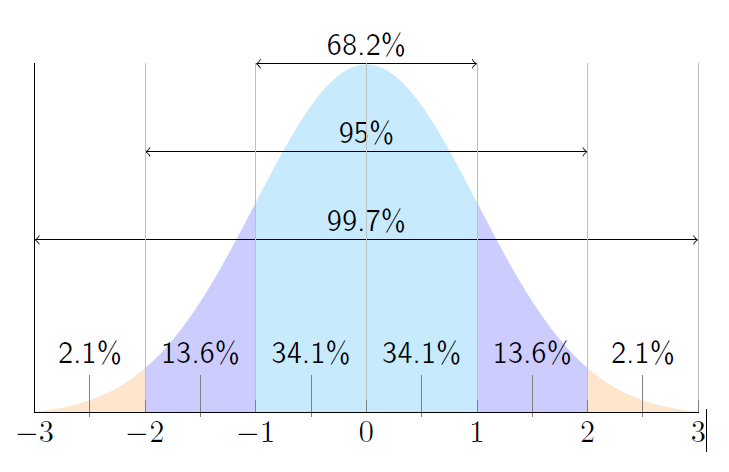
\includegraphics[width=.9\textwidth]
{img/Hoofdstuk_4/GaussCurve.png}
\caption{Standaardnormale verdeling}
\label{fig:GaussCurve}
\end{figure}

De formule voor de standaardnormale verdeling, die te zien is op figuur~\ref{fig:GaussCurve}, is:
\begin{equation}
f(x) = \frac{1}{\sigma \sqrt{2 \pi}} e^{-\frac{1}{2}\frac{(x - \mu)^2}{\sigma^2}}
\end{equation}

Men noteert dat SxS normaal verdeeld is met gemiddelde $\mu$ en standaardafwijking $\sigma$ als: $X \approx Nor(\mu, \sigma)$.

Standaard verdeling: $Z \approx N(\mu = 0, \sigma = 1)$

\begin{enumerate}
\item $N(0,1)$: hiervoor bestaan z-tabellen.
\item Symmetrieregel: $P(Z < -z) = p(Z > z)$
\item 100\% kans: $P(Z < z) = 1- P(Z >z)$
\end{enumerate}

\subsection{De centrale limietstelling}
Als de steekproefomvang voldoende groot is, dan kan de kansverdeling van het steekproefgemiddelde benaderd worden met een normale verdeling.
Dit geldt ongeacht de vorm van de kansverdeling van de individuele waarnemingen.

\subsection{Van steekproef naar populatie}
\subsubsection{Puntschatter}
Een puntschatter voor een populatieparameter is een regel of een formule die ons zegt hoe we uit de steekproef een getal moeten berekenen om de populatieparameter te schatten.

\subsubsection{Betrouwbaarheidsinterval}
Een betrouwbaarheidsinterval is een regel of een formule die ons zegt hoe we uit de steekproef een interval moeten berekenen dat de waarde van de parameter met een bepaalde hoge waarschijnlijkheid bevat.

De betrouwbaarheidscoëfficieënt is de kans dat een willegkeurig gekozen betrouwbaarheidsinterval de parameter bevat.

Het symbool voor betrouwbaarheidscoëfficiënt is $\alpha$.

\paragraph{Voorbeeld:}

We willen betrouwbaarheidsinterval bepalen waar we 95\% dat $\mu$ er in ligt.

$z = \frac{x - \mu}{\frac{\sigma}{\sqrt{n}}}$: Hierbij is $\mu$ onbekend.

We zoeken dus z waarvoor geldt dat:

$P(-z < \mu < +z) = 0.95$

$P(-Z < \mu) = 0.025$ -> $ 0.025 = \frac{\alpha}{2}$

$P(Z > \mu) = 0.025$

$P(-1.96 > \mu) = 0.025$

$P(-1.96 < \frac{\overline{x} - \mu}{\frac{\sigma}{\sqrt{n}}} <1.96)$

$P(\overline{x} - 1.96\frac{\sigma}{\sqrt{n}} < \mu < \overline{x}+1.96\frac{\sigma}{\sqrt{n}})$

Betrouwbaarbeidsinterval: $[x - 1.96\frac{\sigma}{\sqrt{n}} , x+1.96\frac{\sigma}{\sqrt{n}})]$

\subsubsection{Betrouwbaarheidsinterval voor een kleine steekproef}
In plaats van:
$z = \frac{x - \mu}{\frac{\sigma}{\sqrt{n}}}$

construeren we:
$t=\frac{\overline{x}-\mu}{\frac{s}{\sqrt{n}}}$

Om een betrouwbaarheidsinterval voor het gemiddelde te bepalen
op basis van een klein steekproef bepalen we:

$\overline{x} \pm t_{\frac{\alpha}{2}}(\frac{s}{\sqrt{n}})$

waarbij $t_{\frac{\alpha}{2}}$ gebaseerd is op (n - 1) vrijheidsgraden.
We veronderstellen wel dat we een aselecte steekproef genomen hebben uit een populatie die bij benadering normaal verdeeld is.

\subsubsection{Betrouwbaarheidsinterval voor een fractie}
$\overline{p}=\frac{aantal successen}{n}$

\begin{itemize}
\item Verwachting van kansverdeling van $\overline{p} = p$
\item De standaardafwijking van kansverdeling $\overline{p} = \sqrt{\frac{pq}{n}}$
\item Voor grote steekproeven is $\overline{p}$ bij benadering normaal verdeeld.
\end{itemize}
Aangezien $\overline{p}$ een steekproefgemiddelde is van het aantal successen, stelt dit ons in staat een betrouwbaarheidsinterval te berekenen analoog als die voor de intervalschatting van $\mu$ voor grote steekproeven.

\begin{equation}
\overline{p} \pm z_{\frac{\alpha}{2}}\sqrt{\frac{\overline{pq}}{n}}
\end{equation}
met $\overline{p} = \frac{x}{n}$ en $\overline{q}= 1-\overline{p}$

\section{Hypothese toetsen}
\subsection{Toetsen van hypothesen}
Een \textbf{hypothese} is een idee waarvan nog bewezen moet worden dat het juist is.

Een \textbf{hypothesetest} is een vontrole van een uitspraak voer de waarden van één of meerdere populatieparameters.

De \textbf{nulhypothese} ($H_0$) is de hypothese die men probeert te ontkrachten door redenering in het ongerijmde.

De \textbf{alternatieve hypothese} ($H_1$ of $H_\alpha$) is de hypothese die men wil aantonen.

De \textbf{teststatistiek} is de variabele die berekend wordt uit de steekproef.

Het \textbf{aanvaardingsgebied} is het gebied van waarden die de nulhypothese ondersteunt.

Het \textbf{kritieke of verwerpingsgebied} is het gebied van waarden die de nulhypothese verwerpt.

\subsection{Werkwijze}
\begin{enumerate}
\item Bepalen van de hypotheses ($H_0$ en $H_1$)
\item Vastleggen van het significantieniveau ($\alpha$ en $n$)
\item Toestingsgrootheid en waarde ervan bepalen
\item Berekenen en tekenen van het kritieke gebied
\item Conclusies trekken
\end{enumerate}

\subsection{Overschrijdingskans}
De p-waarde is de kans, indien de nulhypothese waar is, om een waarde te verkrijgen van de toetsingsgrootheid die minstens even extreem is al de geobserveerde waarde.

\subsection{Kritieke gebied}
\begin{equation}
g=\mu-z\times \frac{\sigma}{\sqrt{n}}
\end{equation}
Bereken $P(M>g)=\alpha \Leftrightarrow P(Z>\frac{g-\mu}{\frac{\sigma}{\sqrt{n}}})$

\subsubsection{Tweezijdig toetsen}
\begin{equation}
g=\mu \pm z \times \frac{\sigma}{\sqrt{n}}
\end{equation}

\subsection{Samenvatting Z-toets}
\subsubsection{Overschrijdingskans}
\begin{equation}
p=P(Z>\frac{x-\mu_0}{\frac{\sigma}{\sqrt{n}}})
\end{equation}
$P<\alpha \Leftarrow H_0 $ verwerpen.

$P\geq \alpha \Leftarrow H_0$ aanvaarden.
\subsubsection{Kritieke gebied}
\begin{equation}
g=\mu_0 + z\frac{\sigma}{\sqrt{n}}
\label{eq:vergelijkingVoorG}
\end{equation}

In vergelijking~\ref{eq:vergelijkingVoorG} zijn alle waarden buiten z gegeven. Z kan echter makkelijk opgezocht worden in de z-tabel.

\begin{table}[H]
\centering
\begin{tabular}{l c c c}
Doel & \multicolumn{3}{l}{
\begin{minipage}{11cm}
Test op gemiddelde waarde $\mu$ van één populatie a.d.h.v één steekproef van n onafhankelijke steekproefwaarden
\end{minipage}
}\\
\hline
Voorwaarde & \multicolumn{3}{l}{De populatie is willekeurig verdeeld, n voldoende groot ($n>30$)}\\
\hline
Type test & Tweezijdig & Eenzijdig links & Eenzijdig rechts\\
\hline
$H_0$ & $\mu = \mu_0$ & $\mu = \mu_0$ & $\mu = \mu_0$\\
$H_1$ & $\mu \neq \mu_0$ & $\mu < \mu_0$ & $\mu >\mu_0$ \\
Verwerpingsgebied & $|z| > g $ & $z<-g$ & $z>g$\\
Teststatistiek & \multicolumn{3}{l}{$z=\frac{\overline{x}-\mu_0}{\frac{\sigma}{\sqrt{n}}}$} \\
\hline
\end{tabular}
\caption{Samenvatting  voor kritieke gebied}
\label{tab:kritiekeGebied}
\end{table}

\subsection{Conclusies en consequentie bij toetsen van hypotheses}
\begin{table}[H]
\centering
\begin{tabular}{l c c}

& \multicolumn{2}{c}{\textbf{Werkelijke stand van zaken}}\\
\hline
\textbf{Conclusies} & $H_0$ is correct & $H_1$ is correct \\
\textbf{Accepteer $H_0$} & Juist & $2^e$ soort fout ($\beta$)\\
\textbf{Verwerp $H_0$} & Fout van $1^e$ soort & Juist\\
\hline
\end{tabular}
\caption{Conclusies en consequenties bij toetsen van hypotheses}
\label{tab:conseqentiesToetsenHypotheses}
\end{table}

\section{$\chi^2$ Toets}
\subsection{Goodness of fit test}
De goodness of fit test kan gebruikt worden om na te gaan in welke mate de steekproef overeenstemt met een nulhypothese over de verdeling van de variabele.

De verwachte frequenties worden genoteerd met de letter $e$

Er geldt: $e=n\times \pi$

Als de verschillen $o-e$ relatief klein zijn kunnen ze toegerekend worden aan toevallige steekproeffouten.
Hier bij is $o$ de geobserveerde waarde en $e$ de verwachte frequentie.

Beschouw: $\chi^2=\sum^n_{i=1}\frac{(o_i-e_i)^2}{e_i}$

Merk op:

\begin{itemize}
\item indien de verschillen klein zijn $\rightarrow$ verdeling komt voldoende overeen.
\item indien de verschillen groot zijn $\rightarrow$ verdeling is niet representatief
\end{itemize}

\subsection{Toetsingsprocedure goodness of fit test}
\begin{enumerate}
\item Bepalen hypotheses
	\begin{itemize}
	\item $H_0$: steekproef is representatief naar populatie
	\item $H_1$: steekproef is niet representatief naar populatie
	\end{itemize}
\item Bepalen van $\alpha$ en $n$: vaak zelf kiezen of gegeven
\item Toetsinsgrootheid en waarde ervan in steekproef
\item Bereken en teken kritiek gebied: De toets is altijd rechtszijdig
\end{enumerate}

\subsection{Gestandaardiseerde residuen}
De gestandaardiseerde residuen duiden aan welke klassen de grootste bijdrage leveren aan de waarde van de grootheid.

$r_i = \frac{o_i-n\pi_i}{\sqrt{n\pi_i(1-\pi_i}}$

Er geldt algemeen: waarden groter dan 2 of kleinde dan -2 zijn extreem.

\subsubsection{Regel van Cochran}

Om de toets te mogen toepassen dient aan de volgende voorwaarden te zijn voldaan:
\begin{enumerate}
\item Voor alle categorieën moet gelden dat de verwachte waarde $e$ groter is dan 1
\item In ten hoogste 20\% van de categorieën mag de verwachte waarde $e$ kleiner zijn dan 5
\end{enumerate}

\subsection{$\chi^2$ toets voor 2 variabelen}
De Chi-kwadraattoets laat zich eenvoudig uitbreiden tot een onderzoeksontwerp met twee variabelen, met respectievelijk $r$ en $k$ niveaus.

\section{Indexcijfers}
\subsection{Definities}
Een indexcijfer is een getal dat de verandering van een variabele in de loop van de tijd meet in verhouding tot de waarde van de variabele tijdens een bepaalde basisperiode.

$\textnormal{Indexcijfer I} = \frac{uitkomst_{datum}}{uitkomst_{basis}}\times 100\%$

\subsection{Enkelvoudige indexcijfers}
Enkelvoudige indexcijfers hebben betrekking op slechts één object of artikel.

\begin{equation}
I_p = \frac{P-v}{P_b}\times 100
\end{equation}
\begin{equation}
I_q = \frac{Q_v}{Q_b} \times 100
\end{equation}
\begin{equation}
I_w = \frac{P_v \times Q_v}{P_b \times Q_b} \times 100 = \frac{I_p \times I_q}{100}
\end{equation}

\subsection{Samengestelde indexcijfers}
Een samengesteld indexcijfer is het rekenkundig gemiddelde van een aantal enkelvoudige indexcijfers.

\subsubsection{Ongewogen samengestelde indexcijfers}
Aan elk element wordt hetzelfde belang gehecht.
\begin{equation}
\overline{I}=\frac{\sum^n_{i=0}I_i}{n}
\end{equation}
\begin{itemize}
\item $\overline{I}$: ongewogen samengestelde index
\item $I_i$: partiële indexcijfers
\item $n$: aantal partiële indexcijfers
\end{itemize}

\subsubsection{Gewogen samengestelde indexcijfers}
Het belang van de onderscheiden partiële indexcijfers is ongelijk:
men geeft aan elk partieel indexcijfer een wegingscoëfficiënt.

\begin{equation}
\overline{I}= \frac{\sum^n_{i=0}g_i \times I_i}{\sum^n_i g_i}
\end{equation}
\begin{itemize}
\item $\overline{I}$: gewogen samengesteld indexcijfer
\item $g_i$: gewicht of wegingscoëfficiënt van het i$^e$ partiële cijfer
\item $I_i$: partiële indexcijfer
\end{itemize}

\subsubsection{Gewogen gemiddelde van Laspeyres}
Het gewogen samengesteld indexcijfer van Laspeyres is het gewogen gemiddelde van partiële indexcijfers waarbij de
hoeveelheden in de basisperiode constant gehouden zijn m.a.w. indexcijfer met vaste gewichten of berekening volgens basisjaarmethode.

\begin{equation}
I^L_W=\frac{\sum P_v \times Q_v}{\sum P_b \times Q_b}
\end{equation}
Het indexcijfer van Laspeyres geeft antwoord op de vraag: “Welke prijs betaalt men vandaag voor een zelfde hoeveelheid van dezelfde goederen?

\subsubsection{Gewogen samengestelde indexcijfer van Paasche}
Het gewogen samengesteld indexcijfer van Paasche neemt de hoeveelheden in de verslagperiode als wegingcoëfficiënt m.a.w. indexcijfer met veranderlijke gewichten

\begin{equation}
I^P_W=\frac{\sum P_v \times Q_v}{\sum P_b \times Q_b}
\end{equation}

\subsubsection{Kritiek op Laspeyres en Paasche}
Laspeyres' index is een overschatting.

Paasche's index is een onderschatting.

\subsubsection{Gewogen indexcijfer van Fisher}
Fischer’s indexcijfer wordt ook wel eens het ideale indexnummer genoemd voor de volgende redenen:
\begin{itemize}
\item Het is een geometrisch gemiddelde wat als een geschikte maat voor gemiddelde van ratio’s beschouwd wordt.
\item Het neemt zowel de basisjaarhoeveelheden als de huidige hoeveelheden in rekening.
\item Er is geen bias.
\item Het voldoet aan zowel de time reversal als de factor reversal test.
\end{itemize}

= het meetkundig gemiddelde van Laspeyres en Paasches indexcijfer.

\begin{equation}
I^f_W = \sqrt{I^L_W \times I^P_W}
\end{equation}

\section{Tijdsreeksen}
Een tijdreeks is een opeenvolging van observaties van een variabele in functie van de tijd.

Tijdreeksen zijn een belangrijk onderdeel van onderzoek omdat ze vaak de basis vormen voor beslissingsmodellen en voorspellingen.

Tijdreeksen zijn een statistisch probleem: observaties variëren in functie van de tijd.
\subsection{Tijdsreeksmodellen}
\subsubsection{Wiskundig model}
\begin{equation}
X_t = b + \epsilon_t
\label{eq:eenvoudigModelTijdsreeks}
\end{equation}
\begin{itemize}
\item $X_t$ stochastische variabele voor de tijdreeks, op tijdstip $t$
\item $x_t$ observatie op tijdstip $t$
\item $\epsilon_t$ is de storing op een bepaald moment.
\item $\epsilon_t$ wordt verondersteld: $\epsilon_t \approx Norm(\mu=0,\sigma)$
\end{itemize}

\begin{equation}
X_t = b_0 + b_1 \times t + \epsilon_t
\label{eq:lineairVerbandTijdsreeks}
\end{equation}

In vergelijking~\ref{eq:lineairVerbandTijdsreeks} wordt er van een linear verband uit gegaan.

\begin{equation}
X_t=b_0+b_1\times t + b_2 \times t^2 + ... + b_n \times t^n + \epsilon_t
\label{eq:polynomiaalVerbandTijdsreeks}
\end{equation}

In vergelijk~\ref{eq:polynomiaalVerbandTijdsreeks} is het meest algemene verband, het polynomiaal verband. Vergelijken~\ref{eq:eenvoudigModelTijdsreeks} en ~\ref{eq:lineairVerbandTijdsreeks}

\subsubsection{Algemene uitdrukking}
\begin{equation}
X-t = f(b_0,b_1,b_2 ... b_n,t)+\epsilon_t
\label{eq:AlgemeneUitdrukkingTijdreeks}
\end{equation}

We gaan verder uit van deze veronderstellingen:
\begin{itemize}
\item we beschouwen twee componenten van variabiliteit
	\begin{itemize}
	\item het gemiddelde van de voorspellingen verandert in de tijd
	\item de variaties ten opzichte van dit gemiddelde variëren willekeurig
	\end{itemize}
\item De variatie van de residuen van het model $(X_t - x_t)$ is constant in de tijd
\end{itemize}

\subsubsection{Schatten van de parameters}
Voorspellingen maken aan de hand van tijdreeksmodel:
\begin{enumerate}
\item Selecteer het meest passende model
\item Schatting voor parameters $b_i(i:1..n)$ a.d.h.v. observaties
\end{enumerate}
Deze schattingen $\hat{b_i}$ zijn dan zodanig dat ze de geobserveerde waarden zo goed mogelijk benaderen.

\subsection{Vooruitschrijdend gemiddelde}
\subsubsection{Eenvoudig vooruitschrijdend gemiddelde}
Het eenvoudig voortschrijdend gemiddelde is een reeks gemiddelden van de laatste $m$ observaties.

Het vooruitschrijden gemiddelde wordt vaak afgekort tot SMA (Simple Moving Average).

$SMA(t) = \sum^t_{i=k}\frac{x_i}{m}$ met $k = t-m+1$

Hierbij is m het tijdsbereik.

SMA verbergt korte termijn fluctuaties en tonen lange termijn trends

\subsubsection{Gewogen vooruitschrijdend gemiddelde}
Bij gewogen vooruitschrijdend gemiddelde (WMA: Weighted Moving Average) wegen recentere observaties meer door.

Een specifieke vorm hiervan is exponentiële afvlakking of het exponentieel vooruitschrijdend gemiddelde (EMA).

$EMA(t) = \alpha x_{t-1} + (1-\alpha ) EMA(t-1)$

met $\alpha$ de smoothing constante ($0<\alpha < 1$) en $t\geq 3$

Er wordt voor exponentieel gekozen omdat oudere observaties een exponentieel kleiner gewicht krijgen.

\subsubsection{Dubbele exponentiële afvlakking}
We voeren een extra term in om de trend te modelleren.
We noteren $s_t$ voor de afgevlakte waarde, en $b_t$ voor de schatting van de trend op tijdstip $t > 1$:

$s_t = \alpha w_t + (1-\alpha ) (x_{t-1}+b_{t-1})$

$b_t = \beta (s_t - s_{t-1})+(1-\beta )b_{t-1}$

met $0 < \alpha < 1$ en $0 < \beta < 1$

Voor $s_1$ wordt vaak $x_1$ gekozen.
Voor $b_1$ zijn er meerdere mogelijkheden.

\textbf{Voorspellen}

Om een voorspelling $F(t+1)$ te maken voor tijdstip $t+1$ gebruiken we:

$F(t+1) = s_t +b_t$

of in het algemen voor tijdstip $t+m$:

$F(t+m) = s_t + mb_t$

\subsubsection{Driedubbele exponentiële afvlakking}
Deze methode wort ook vaak \textit{de methode van Holt-Winters} genoemd.
Deze houdt rekening met seizoenaliteit in de data.
We noteren:
\begin{itemize}
\item $L$: lengte van de seizoenale cyclus (aantal tijdseenheden)
\item $c_t$: term die de seizoenale variaties modelleert
\item $\gamma$: smoothing factor voor de seizoenale variatie
\end{itemize}

\begin{equation}
\begin{array}{rcl}
s_0 & = & x_0\\
s_t & = & \alpha\frac{x_t}{c_{t-L}}+(1-\alpha)(s_{t-1}+b_{t-1})\\
b_t & = & \beta(s_t-s_{t-1})+(1-\beta)b_{t-1}\\
c_t & = & \gamma\frac{x_t}{s_t}+(1-\gamma)c_{t-L}\\
\end{array}
\end{equation}

\textbf{Voorspelling}

Voorspellingen op tijdstip $t+m$:

$F_{t+m}=(s_t+mb_t)c_{t-L+1+(m-1)}\:mod\:L$
\end{document}